%%%%%%%%%%%%%%%%%%%%%%%%%%%%%%%%%%%%%%%%%%%%%%%%%%%%%%%%%%%%%%%%%%%%%%%%%%%%%%%%
%2345678901234567890123456789012345678901234567890123456789012345678901234567890
%        1         2         3         4         5         6         7         8

%\documentclass[letterpaper, 10 pt, conference]{ieeeconf}  % Comment this line out
                                                          % if you need a4paper
\documentclass[a4paper, 10pt, conference]{ieeeconf}      % Use this line for a4
                                                          % paper

\IEEEoverridecommandlockouts                              % This command is only
                                                          % needed if you want to
                                                          % use the \thanks command
\overrideIEEEmargins
% See the \addtolength command later in the file to balance the column lengths
% on the last page of the document

\usepackage[pdftex]{graphicx}
\usepackage[usenames,dvips,pdftex]{color}
\usepackage{wrapfig}
\usepackage{multicol}
\usepackage{amsmath, amsfonts}
\usepackage[nice]{nicefrac}
\usepackage{longtable}
\usepackage{wrapfig}
\usepackage{cite}
\usepackage{units}
\usepackage{url}
%\usepackage[noend]{sty/algorithmic}



% The following packages can be found on http:\\www.ctan.org
%\usepackage{graphics} % for pdf, bitmapped graphics files
%\usepackage{epsfig} % for postscript graphics files
%\usepackage{mathptmx} % assumes new font selection scheme installed
%\usepackage{times} % assumes new font selection scheme installed
%\usepackage{amsmath} % assumes amsmath package installed
%\usepackage{amssymb}  % assumes amsmath package installed

\title{\LARGE \bf
Learning Real Scale of Object Instances And Categories Scale Distributions from CAD Models
}

%\author{ \parbox{3 in}{\centering Huibert Kwakernaak*
%         \thanks{*Use the $\backslash$thanks command to put information here}\\
%         Faculty of Electrical Engineering, Mathematics and Computer Science\\
%         University of Twente\\
%         7500 AE Enschede, The Netherlands\\
%         {\tt\small h.kwakernaak@autsubmit.com}}
%         \hspace*{ 0.5 in}
%         \parbox{3 in}{ \centering Pradeep Misra**
%         \thanks{**The footnote marks may be inserted manually}\\
%        Department of Electrical Engineering \\
%         Wright State University\\
%         Dayton, OH 45435, USA\\
%         {\tt\small pmisra@cs.wright.edu}}
%}

\author{Aitor Aldoma, Walter Wohlkinger and Markus Vincze% <-this % stops a space
\thanks{This work was not supported by any organization}% <-this % stops a space
\thanks{H. Kwakernaak is with Faculty of Electrical Engineering, Mathematics and Computer Science,
        University of Twente, 7500 AE Enschede, The Netherlands
        {\tt\small h.kwakernaak@autsubmit.com}}%
\thanks{P. Misra is with the Department of Electrical Engineering, Wright State University,
        Dayton, OH 45435, USA
        {\tt\small pmisra@cs.wright.edu}}%
}


\begin{document}



\maketitle
\thispagestyle{empty}
\pagestyle{empty}


%%%%%%%%%%%%%%%%%%%%%%%%%%%%%%%%%%%%%%%%%%%%%%%%%%%%%%%%%%%%%%%%%%%%%%%%%%%%%%%%
\begin{abstract}

This paper presents a method to automatically learn a scaled CAD model representation
of object instances seen by a depth sensor. The CAD models representing objects belonging to different categories
are downloaded automatically from the Internet. When an object is placed in front of the camera, the system tries
to recognize it and estimate their pose against the already learned CAD models using a fast scale-dependant 3D feature. Upon failure, a learning stage is triggered that
categorizes the object using a scale invariant view based descriptor to retrieve CAD models from the categories database with
similar geometries as seen from the sensor viewpoint. The retrieved CAD models are fitted against the partial view of the object, 
the model that best fits the partial view is selected and a scaled version of model that fits the object instance is stored for future recognition. Moreover, after
a certain amount of object instances has been learned, the system learns a scale distribution for each category that can be used to filter false
positives based on the already-learned distribution to improve the efficiency of the learning stage. This approach has several advantages over: (i) high-precission scanners as they
have a high cost and the scanning process is cumbersome and (ii) mesh reconstruction methods based on images or fusion of partial views regarding accuracy and completeness of the
CAD model. We demonstrate the use of this approach to learn a set of object instances and present recognition and pose estimations results using the scale invariant semi-global
3D feature CVFH.

\end{abstract}


%%%%%%%%%%%%%%%%%%%%%%%%%%%%%%%%%%%%%%%%%%%%%%%%%%%%%%%%%%%%%%%%%%%%%%%%%%%%%%%%
\section{INTRODUCTION}

%%%%%%%%%%%%%%%%%%%%%%%%%%%%%%%%%%%%%%%%%%%%%%%%%%%%%%%%%%%%%%%%%%%%%%%%%%%%%%%%

\section{FRAMEWORK}

\onecolumn
\begin{figure}[htb]
  \begin{center}
    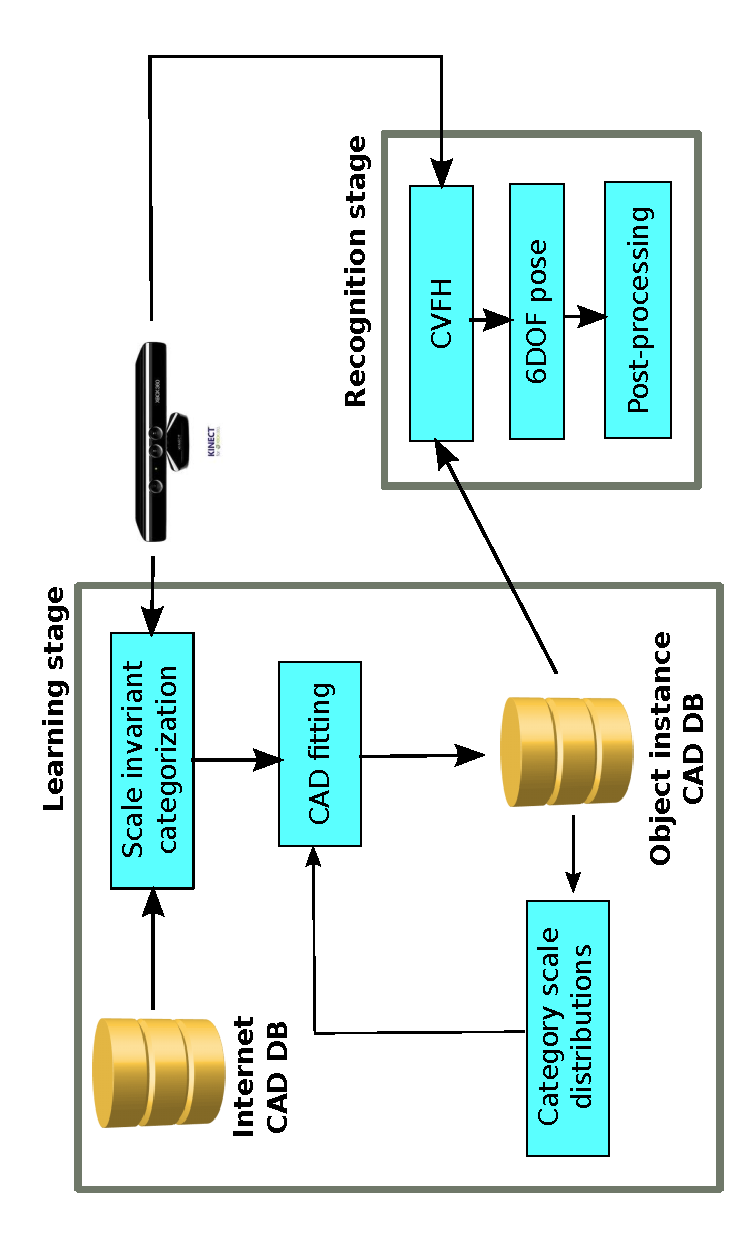
\includegraphics[angle=270,width=\columnwidth]{images/framework.pdf}
    \caption{Framework}
    \label{fig:framework}
  \end{center}
\end{figure}

\twocolumn

\section{LEARNING STAGE}

\subsection{Categorization}

\subsection{CAD model fitting}

\section{CATEGORIES SCALE DISTRIBUTION}

\section{SCALE DEPENDANT RECOGNITION AND POSE ESTIMATION}

\section{EVALUATION}

The CAD model database from the Internet contains approx. $8000$ objects belonging
to $200$ categories published online ...

We evaluate the system in two ways: (i) we select $20$ real objects. We manually search for each real object  and at the same time learn them using categorization and stable pose
alignment obtaining . We can then evaluate if 

(ii) we try to learn $50$ objects
belonging to $5$ different categories using the scale invariant categorization
method and stable pose alignment presented befofe and we use the learned models
to perform recognition and pose estimation on several scenes containing this objects using CVFH.

%%%%%%%%%%%%%%%%%%%%%%%%%%%%%%%%%%%%%%%%%%%%%%%%%%%%%%%%%%%%%%%%%%%%%%%%%%%%%%%%
\section{ACKNOWLEDGMENTS}

The authors gratefully acknowledge the contribution of National Research Organization and reviewers' comments.


%%%%%%%%%%%%%%%%%%%%%%%%%%%%%%%%%%%%%%%%%%%%%%%%%%%%%%%%%%%%%%%%%%%%%%%%%%%%%%%%

References are important to the reader; therefore, each citation must be complete and correct. If at all possible, references should be commonly available publications.

\begin{thebibliography}{99}

\bibitem{c1}
J.G.F. Francis, The QR Transformation I, {\it Comput. J.}, vol. 4, 1961, pp 265-271.

\bibitem{c2}
H. Kwakernaak and R. Sivan, {\it Modern Signals and Systems}, Prentice Hall, Englewood Cliffs, NJ; 1991.

\bibitem{c3}
D. Boley and R. Maier, "A Parallel QR Algorithm for the Non-Symmetric Eigenvalue Algorithm", {\it in Third SIAM Conference on Applied Linear Algebra}, Madison, WI, 1988, pp. A20.

\end{thebibliography}

\end{document}
